\documentclass[nofilelist]{cslthse-msc}
% to show a list of used packages at the end of the document, delete the nofilelist option
%\documentclass{cslthse-msc} 
\usepackage[utf8]{inputenc}
\usepackage[english]{babel}
\usepackage{amsmath}
%\usepackage{amsfonts}
%%\usepackage{amssymb}
\usepackage{amsthm}
%\usepackage{makeidx}
\usepackage{graphicx}
\usepackage[titletoc, header, page]{appendix}
\usepackage{transparent}
\usepackage{natbib}
\usepackage{wrapfig}
\usepackage{amsmath}
\usepackage{multirow}
\usepackage{tabularx}
\usepackage{subfig}
\usepackage{textcomp}
\usepackage{calligra}
\usepackage{nameref}
\usepackage{float}




\newcommand{\icon}[1]{
\includegraphics[height=30pt]{msccls/explanatory_images/CASTLE_logo.png}}

% used to display the used files at the end. Select nofilelist as a package option to disable this
\listfiles % initialize

%\geometry{showframe}
%better like this?
%\student{Flavius Gruian}{Flavius.Gruian@cs.lth.se}
\students{Nick Persson}{nick@persson.dev}{Filip Karabeleski}{fkarabeleski@gmail.com}

\thesisnumber{LU-CS-EX: 2021-XX} % Birger Swahn will provide this number to you, once the thesis is ready for publication
% default is Master. Uncomment the following for "kandidatarbete"/Bachelor's thesis
%\thesistype{Bachelor}{Kandidatarbete}

%\title{Formatting a Master's Thesis}
\title{Emotion Recognition in Written Conversations Using CASTLE}

%\onelinetitle
%\twolinestitle
\threelinestitle
%\fourlinestitle

\subtitle{\protect\icon{CASTLE}}
\company{Telavox AB}
\supervisors
{Sara Lindgren, \href{mailto:Sara.Lindgren@telavox.com}{\texttt{Sara.Lindgren@telavox.com}}}
{Pierre Nugues, \href{mailto:Pierre.Nugues@cs.lth.se}{\texttt{Pierre.Nugues@cs.lth.se.com}}}
\examiner
{Flavius Gruian, \href{mailto:Flavius.Gruian@cs.lth.se}{\texttt{Flavius.Gruian@cs.lth.se}}}

\date{\today}
%\date{January 16, 2015}

\acknowledgements{


We would like express our gratitude, first and foremost, to our supervisor Pierre. There is no way that this project would have been completed without your guidance, at least not in time. 


We would also like to thank \textit{Telavox} and our company supervisor Sara for our weekly meetings, where much of our planning and reflection were made. 


As the COVID-19 epidemic created some unusual circumstances, we would like to give a special thanks to \textit{Åke P Fågel \& Vilt} for providing us with a stable office to work out of. 
}

\theabstract{
%This document describes the Master's Thesis format for the theses carried out at 
%the Department of Computer Science, Lund University. 

%Your abstract should capture, in English, the whole thesis with focus on the problem and solution in 150 words. It should be placed on a separate right-hand page, with an additional \textit{1cm} margin on both left and right. Avoid acronyms, footnotes, and references in the abstract if possible.


%Leave a \textit{2cm} vertical space after the abstract and provide a few keywords relevant for your report. Use five to six words, of which at most two should be from the title.
}

\keywords{Machine Learning, NLP, Emotion Recognition}

%% Only used to display font sizes
\makeatletter
\newcommand\thefontsize[1]{{#1 \f@size pt\par}}
\makeatother
%%%%%%%%%%

\begin{document}
\renewcommand{\bibname}{References}

\makefrontmatter
\chapter{Introduction}

%ML är automagiskt - PopSci

\section{Background}
Natural language processing (NLP) is a field of study mainly in computer science that deals with analyzing human language in a way that computers can understand and process. According to \citet{ntlk2009}, natural language is used for everyday communication by humans, in contrast to artificial languages such as programming languages and mathematical notation. Since natural languages naturally evolve as time goes on and their adherence to structure diminish, it is difficult to define explicit rules to follow. For this reason, there is a need for machine learning models to aid the computer in identifying these diffuse rules. 

In order to feed the model with effective information, the input is structured and inserted into a data set. This way, the computer has an easier way of processing and analyzing the data. When handling data sets constructed using exclusively textual input, the data sets are instead referred to as \textit{corpora}. 

%?? and hence the need of machine learning to replace rules?? ?? You need also to introduce more specifically your task ??



\section{Purpose}
Customer service is centered around the relation between company and customer with the goal of pleasing the customer. This goal can be very difficult to achieve and there is no straightforward way to do so. By analyzing prior conversations, it is possible for companies to gain valuable insights in the most effective way to please the customer. Customer service is however a massive industry and it would take countless hours to analyze the conversations from even a single company manually. 

The company sponsoring this project approached us with an idea to try and solve this problem using machine learning. A usual technique for these types of problems is \textit{sentiment analysis}, where utterances are labeled either as positive or negative. We instead decided to take another route, namely \textit{emotion recognition}. Emotion recognition focuses on labelling utterances from a non-binary set of emotions instead of sentiment analysis' binary method. This allows an analysis with greater specificity.  

In order to further the academic relevance of this project we decided that we would attempt to contribute to the field of emotion recognition by achieving state-of-the-art results. 

\section{State-of-the-art}
In this paper, the term state-of-the-art will be recurringly mentioned as it is a fundamental part of our aim and result. The term refers to the highest level of achievement accomplished. A common goal in machine learning projects is to attempt to raise the bar for the current state-of-the-art results across various metrics for the task that the project is trying to solve. Presenting state-of-the-art results is an excellent approach in proving that an implementation or algorithm is valid and valuable.   

%Description of what it is and why it plays a big part in advancing algorithms and models. Deepminds Alphafold has led to groundbreaking results in a competitive environment. 


\section{Telavox}
We carried out this project at Telavox AB. Telavox is a Swedish telecommunication company that specializes in business-to-business and business-to-customer unified communication as a service. As all of their customers deal in customer service, they would all benefit from the solution previously discussed. Telavox therefore has a great interest in being able to offer this as a service. As Telavox has over 250 businesses as customers, the solution would facilitate the quality of customer service world wide.





\section{Research questions}
\label{research_questions}
The primary aim of this thesis is to create a emotion recognition model that is able to produce state-of-the-art results. After this, a secondary aim is to investigate whether or not it is possible to create a dynamic model for instant response regarding customer service related conversations. The following questions are used as guidelines on how to realize these aims.  

\begin{itemize}
    \item \textit{Is it possible to create a model that fulfills our aims?}
%?? THe first question is can we create such a model??
    \item \textit{Could a different architecture than the current state-of-the-art produce better results?}
%?? here your statement is too specific as you did not introduce the terms. Use vague words such as What are the different option to design an architecture and train a model?? 
%?? I have swapped the items ??
    \item \textit{How does our model compare to other models in the same field evaluating on the same metrics?}
    \item \textit{After implementing a fully functioning model, how can we adapt it to predict utterances in real-time?}
    %Snacka om detta i limitations
\end{itemize}




%NLP, ML, Speech-to-text och (STT), API. Modality. RNN, GRU, LSTM, BPTT(?), utterance, speaker, dialogue, 

%Hyperparameters en punkt i listan, items i hyperparameters en sublist

%Kan också kallas för Glossary and Abbreviations






\chapter{Theory}

The celebrity of computer science at this time is undoubtedly \emph{artificial intelligence} (AI). A much more complex subject than most people know. Most of the complex problems in AI are solved using technologies within its sub-fields, which are illustrated in Figure \ref{fig:map}, rather than traditional artificial intelligence such as robotics \citep{bajwa_2020}. 

%In order to solve most emotion recognition problems, there are two main concepts that are fundamental to build an accurate model. Firstly, the model should be created with deep learning algorithms. This enables it to find patterns that it otherwise could not be able to. Secondly, to effectively process the utterances it has been tasked to analyze, a word vector is often used to store the most commonly used words for easier analysis. ?? I propose this instead??

In order to solve most emotion recognition problems, there are two main concepts that are fundamental to build an accurate model:
\begin{enumerate}
\item As shown by the recent progress in the field \citep{deep_survey}, the model should be created with deep learning algorithms. This should enable it to find patterns that it otherwise could not be able to. 
\item To effectively process the utterances, deep learning requires to collect an annotated corpus and design an appropriate representation for the words.
\end{enumerate}


\begin{figure}[h!]
    \centering
    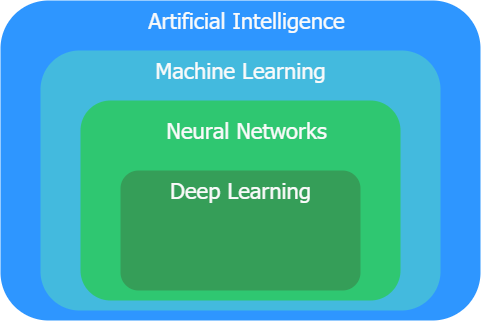
\includegraphics[scale=0.4]{msccls/explanatory_images/map_of_techniques.png}
    \caption{Relations between the related fields of study }
    \label{fig:map}
\end{figure}

\section{Machine Learning}
Machine learning \citep{franoischollet2017learning} is a field of study in artificial intelligence that aims to train a system to solve a problem, rather than to explicitly program the system. By being presented with large amounts of data associated with the task at hand, the system algorithmically builds a statistical model that discovers structures in the data and allows the system to identify rules for the problem. 
In \textit{supervised learning} \citep{100pageBurkov}, which is one of the two main types of tasks in machine learning, the dataset is the collection of labeled examples $\{(\mathbf{x}_i, y_i)\}_{i=1}^N.$ Each element $\mathbf{x}_i$ is a feature vector that contains a value describing the example somehow and $y_i$ is a label, which is either a finite set of classes or a real number. The purpose of supervised learning is to use the dataset to produce a model that takes a feature vector $\mathbf{x}$ as input and outputs information that allows deducing the label $y$ for this feature vector.) 

The other main type of task in machine learning is \textit{unsupervised learning}. The dataset for unsupervised learning is $\{ (\mathbf{x}_i)\}_{i=1}^N$ where $\mathbf{x}_i$ is a feature vector. The goal of unsupervised learning is to use the dataset to produce a model that takes a feature vector $\mathbf{x}$ as input and outputs either another vector or a value. 





\subsection{Neural Networks and Deep Learning}

Neural networks are machine learning systems loosely inspired by biological neural networks. A neural network is a collection of connected nodes or neurons that was first mentioned in \citet{mcculloch1943}. A neuron \citep{dawson1998ann} is an information-processing unit that receives multiple inputs and produces a single output that can be sent to multiple other neurons. To find the output of a neuron the weighted sum of all inputs is weighted by the weights all connecting to the neuron. This weighted sum is then passed through an activation function to provide the output.


%Weights control the signal (or the strength of the connection) between two neurons. In other words, a weight decides how much influence the input will have on the output.


\begin{figure}[htp]
    \centering
    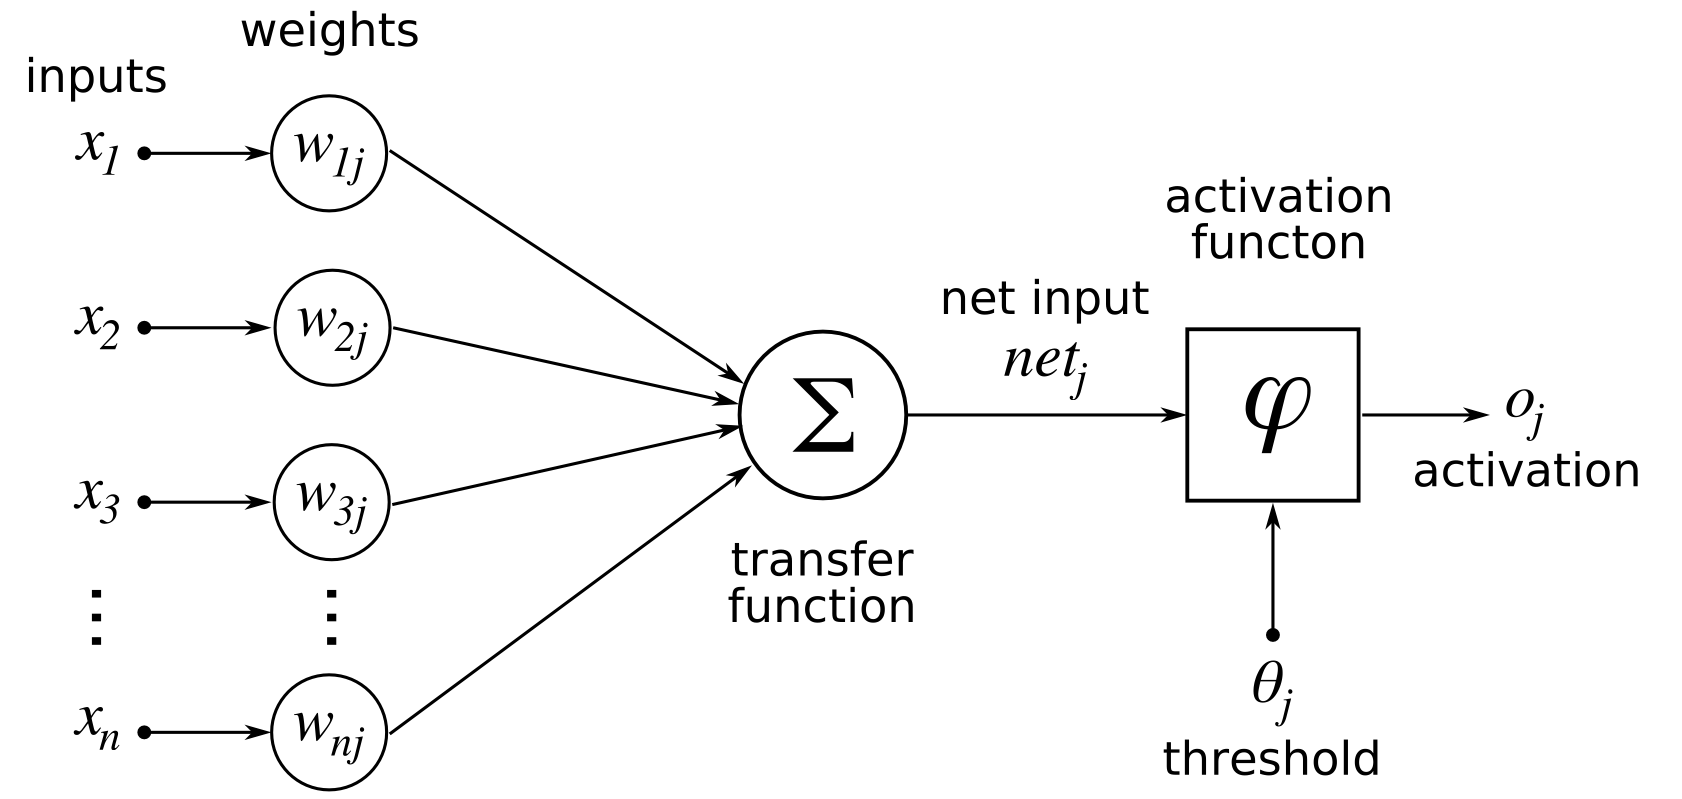
\includegraphics[width=12cm]{msccls/explanatory_images/neuron_new.png}
    \caption{An example of a single neuron. From \citet{wiki:neuron_image}.}
    \label{fig:neuron}
\end{figure}


\begin{equation}
    g(x_1, x_2, x_3,...,x_n) = g(x) = \sum_{i=1}^n  xi
\end{equation}

Here, $g(x)$ takes the inputs $x_1, x_2, x_3,...,x_n$, while the activation function $f(x)$ defines the output. An example of a well known activation function is \textit{ReLU}, Rectified linear unit, which has the following function. 

\begin{equation}
y = f(g(x)) =
\begin{cases}
  0, & \text{if}\ x \leq 0 \\
  x, & \text{if}\ x > 0
\end{cases}
\end{equation}

Neural networks can in turn be structured together and form multiple layers that progressively learn. These networks fall under the deep learning umbrella. Deep learning has several closely related definitions, where \citet{deng2014deep} mentions the following:

\begin{quote}{A class of machine learning techniques that exploit many layers of non-linear information processing for supervised or unsupervised feature extraction and transformation, and for pattern analysis and classification.}
\end{quote}

Each of the layers in a deep learning network manipulates its input data in some way, and the result is stored in the layer's weights. The results are monitored with the help of the \textit{loss function}. The loss function returns a distance score that indicates how far off the network's previous prediction was from the true values \citep{franoischollet2017learning}. The concept of reducing the distance score that the loss function produces is called training.

Using the score produced by the loss function as feedback, the \textit{backpropagation} algorithm computes the \textit{gradient}, a multi-variable generalization of the derivative, which is then used to adjust the weights in such a way that the distance score produced by the loss function is minimized. 


\subsection{Recurrent Neural Network -- RNN}

One of the simplest neural network classes used in deep learning is \emph{recurrent neural networks} (RNN). RNN process either sequential data or time-series data \citep{lipton2015critical}. Since the inputs are sequential, all the inputs are dependent on each other in one way or another. RNNs are therefore suitable for processing sequences of text, audio, and video where every computation will be performed on each element in the sequence.

One of RNN's weaknesses is that they suffer from the \textit{vanishing gradient problem} \citep{hochreiter1998}. While RNN's theoretically can process arbitrarily long sequences, in practice, they are limited to the length of the sequence. If the sequence is too long, the network will struggle to try to look back in time longer than a few steps away. In a lot of cases, this will result in leaving out important information from the prediction. There are instead other alternatives that consider this weakness. 


%Time series. Meant to process sequences of data like text, audio, video. Neural networks that feed their output back into their inputs recursively. One of the more basic building blocks in machine learning/deep learning. A gate looks like this: 

%suffer from short-term memory. If a sequence is long enough, they’ll have a hard time carrying information from earlier time steps to later ones. So if you are trying to process a paragraph of text to do predictions, RNN’s may leave out important information from the beginning.
 
 \begin{figure}[H]
    \centering
    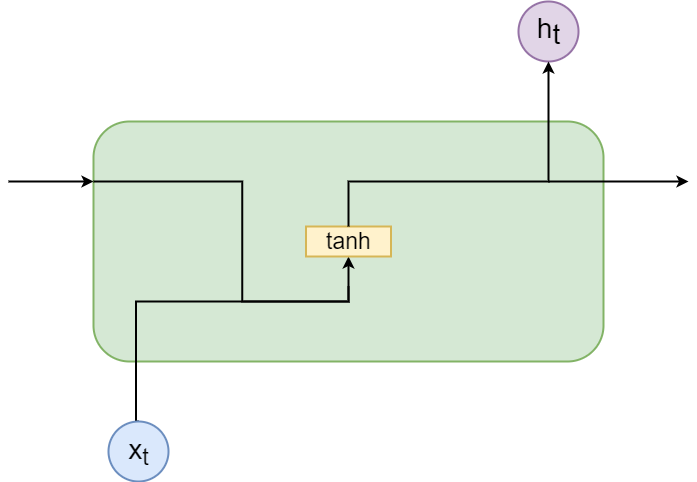
\includegraphics[scale=0.35]{msccls/explanatory_images/rnn.png}
    \caption{A simple RNN node}
    \label{fig:rnn_node}
\end{figure}



\subsection{Long Short-Term Memory -- LSTM}
%?? I would have this section before GRU ??

Another widely used recurrent neural network architecture is Long Short-Term Memory (LSTM). It was proposed by \citet{hochreiter1997} as a solution to the vanishing gradient problem that might occur in recurrent neural networks and has barely been changed since. The vanishing gradient problem occurs in machine learning when the gradient progressively decreases, which prevents the adjustments of the weight's values. 


As illustrated in Figure \ref{fig:lstm_node}, a LSTM node consists of an \textit{input gate}, an \textit{output gate}, a \textit{forget gate} and a \textit{cell state}. 
\begin{itemize}
    \item The input gate controls the extent of data to write onto the internal cell-state.
    \item The output gate controls the extent of data to pass as output. 
    \item The forget gate that decides how much of the previous data is irrelevant and will be ignored. 
    \item The cell state stores the previous state of a node and passes it on to its following node. 
\end{itemize}




\subsection{Gated Recurrent Unit -- GRU}
%Byta alla "node" till "cell" för att lättare kunna referera till LSTM-celler i CASTLE
A \emph{gated recurrent unit} (GRU) is recurrent neural network architecture introduced by \citet{cho2014learning} and is considered an improvement to the traditional recurrent neural networks. 

Basic GRU nodes  are primarily constructed of an \textit{update gate} and a \textit{reset gate}. The update gate regulates the amount of information that is passed along to the next state, while the reset gate, much like the forget gate of LSTM, decides the amount of past information that is going to be disregarded henceforth. 

Although fairly new, it is already a well-established variant of recurrent neural networks. In comparison to \textit{LSTM} layers, GRU layers are cheaper to run since they use fewer parameters, but have less representational power. It has been shown by \citet{Gruber2020AreGC} that GRU layers have had better performance on smaller and less frequent datasets than LSTM layers.

%?? You cannot cite LSTM without describing them first. In addition GRU are newer than LSTMs??

\begin{figure}[!ht]
    \centering
    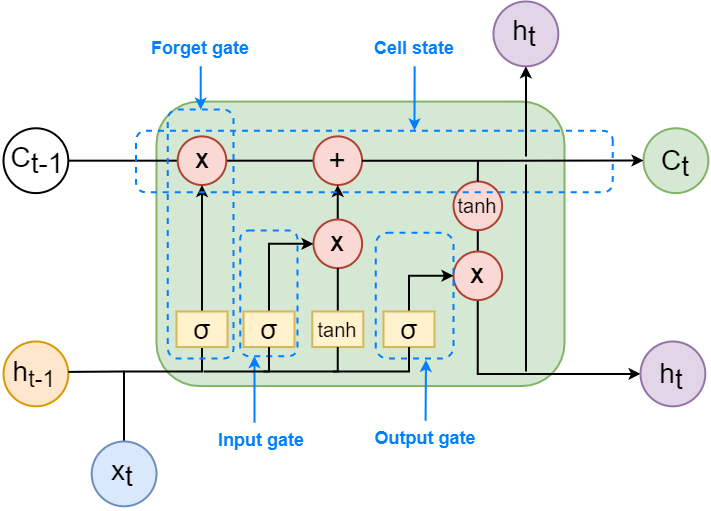
\includegraphics[scale=0.58]{msccls/explanatory_images/lstm.png}
    \caption{A LSTM node} 
    %?? You need to mention the source of your figure if it is not yours??
    \label{fig:lstm_node}
\end{figure}

\begin{figure}[!ht]
    \centering
    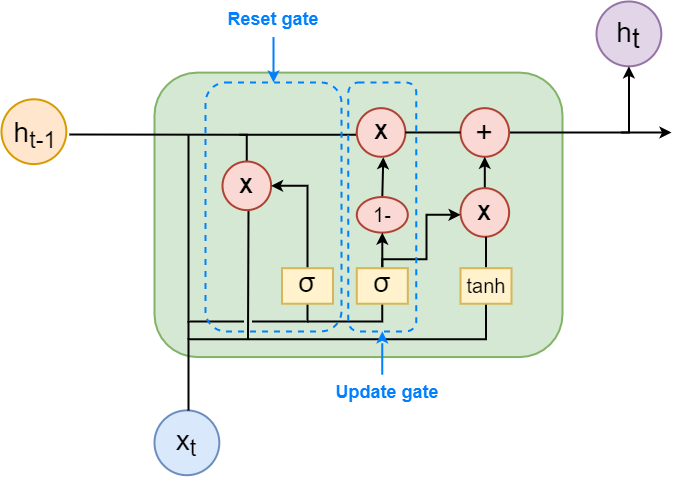
\includegraphics[scale=0.58]{msccls/explanatory_images/gru.png}
    \caption{A GRU node}
    \label{fig:gru_node}
\end{figure}


\section{Training Process}
In order to train a model, there must exist some data set, either labeled or unlabeled depending on whether supervised or unsupervised learning is the targeted method, that feeds the model with input. When using a labeled data set, the labels are regarded as the solution to the problem. When training a model, the goal is to find values for its weights such that the model correctly labels the given input. 

The training of a model is done step by step in the form of \textit{epochs}. Epochs represent the number of times that the model iterates through a data set that is intended to train the model. Following each epoch, a \textit{loss function} measures how incorrect the model's previous prediction was and produces a value for the \textit{loss}. The model will have a perfect prediction when the loss reaches zero, therefore minimizing the loss is desirable. 

The \textit{backpropagation} algorithm is a fundamental tool for minimizing the loss. The algorithm starts with the loss and works its way \textit{backwards} through the layers of the network and applies the chain rule to determine how much impact each of the weights has had on the loss. This impact is then used for the \textit{gradient descent} algorithm to alter the weights in the direction of flattening out the derivative. While travelling through the function, the ultimate goal is to find where the derivative is zero and this is done for each weight in the network. Gradient descent updates the weights to match the results from the backpropagation algorithm \citep{franoischollet2017learning}. 

%bild på training process

%Man får inte minimera lossen för aggressivt, det finns en balans, annars sker overfitting vilket är......
%When training a model 
%Overfitting is a concept in statistical analysis in which the  model fits well on the training set but fails when introducing new examples. Instead of the model learning how to notice and predict features, it simply remembers an unreasonable amount of examples from the training set. This causes the model to perform very well on that specific data but would likely have a very high error rate on any unseen data. 

%bild på overfitting







\section{Evaluation}
Many different metrics can be used to evaluate a machine learning model, based on what kind of model and what its purpose is. For classification models, many of the metrics are based on a confusion matrix \citep{FAWCETT2006861}. 

In a confusion matrix, one of the axes represents the actual class of the instance the model is trying to predict and the other represents what instance the model predicted. The most basic and common confusion matrix is a binary $2 \cdot 2$ matrix, as seen in Figure \ref{fig:confusion}. In binary cases, the instances usually can be represented as a yes or no question, such as \textit{is there a bird in this picture?}

\begin{figure}[h!]
    \centering
    \hbox{\hspace{6em}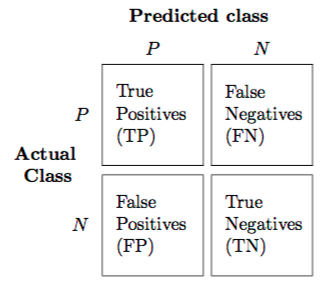
\includegraphics[width=\textwidth/2]{msccls/explanatory_images/confusion_matrix.png}}
    \caption{Binary Confusion Matrix}
    \label{fig:confusion}
\end{figure}

\begin{itemize}
    \item TP means that the model was correct in predicting positive
    \item TN means that the model was correct in predicting negative
    \item FP means that the model was incorrect in predicting positive
    \item FN means that the model was incorrect in predicting negative
\end{itemize}

Whenever our model predicts an instance during training, we increment the corresponding cell in the matrix, letting us see and draw conclusions based on how our model performed. 


For cases where we have multi-class classification instead of binary, such as when determining emotions, the same logic and matrix is used but on a bigger scale and with the specific classes instead of positive and negative. 

The equations provided in subsequent sections to display how to calculate metrics are identical for multi-class context, but the classification instead represents the sum of the classification for each class. For instance, when determining if an emotion is \textit{Neutral}, \textit{Happy}, or \textit{Angry}, $TP_{neutral}$ would represent when it got neutral correct, and TP would be the sum of all emotion predictions it got correct.  



%kan snacka om Type I och Type II errors om mer text behövs.






\subsection{Accuracy}
Accuracy quantifies how many percent of predictions the model got right and is calculated by taking all instances, where our model predicted positive and dividing it with all instances:

$$ Accuracy = \frac{TP + TN}{TP + TN + FP + FN}$$

If we have a balanced dataset with a similar amount of positive and negative instances, then this can give valuable information on the performance of the model since getting predictions right is the goal of any model. If, however, our set is imbalanced and contains e.g. 90 percent negative instances and only 10 percent positive, the model can achieve a 90 percent accuracy by simply predicting negative on every instance so the accuracy suddenly becomes useless \citep{imbalancedlearning}. 

\subsection{Precision}
Precision is a metric that quantifies how many of the instances predicted positive that were true. It's calculated by taking all of the instances where the model predicted positive and was correct and dividing it by all the instances where it predicted positive.

$$ Precision = \frac{TP}{TP + FP}.$$

Precision gives us information on how correct the model is when predicting an instance to be true. This is useful when dealing with instances, where it's important to not give a false positive. If we have a model that is trying to predict whether or not a suspect is guilty of a certain crime, a high precision would make it unlikely for an innocent person to be determined as a criminal. 

However, precision does not give any information on the number of false negatives present, meaning that a high precision could mean that the model seldom identifies a person, but when it does identify someone, that said person is likely guilty.

\subsection{Recall}
Recall is a metric that quantifies how many percent of positive instances that our model managed to predict which we calculate by dividing all instances the model predicted positive and was right by all positive instances.

$$ Recall =\frac{TP}{TP + FN}.$$

As a sort of counterpoint to precision which tells us how good the model is when guessing true, recall tells us how many positive instances the model missed. A high recall can be extremely important when dealing with subjects such as contagious diseases where a result of false-negative can be devastating. 

Recall does not take into account how many positive predictions turned out to be false so in cases, where that does not matter and you want to predict positive at the slightest probability of it being true, optimizing for a high recall is essential.


\subsection{F1 score}
A combination of the two previous metrics, the F1 score, is calculated by creating the harmonic mean of precision and recall:

$$ F1score = 2 \cdot \frac{Precision \cdot Recall}{Precision + Recall}.$$

In cases where there is no extra cost associated with either false negatives or false positives, the goal is usually to minimize the total amount of errors. The harmonic mean is a type of average that is appropriate when working with ratios, which is what both precision and recall are. 

This lets us improve the model concerning either of the variables and not have to think about if, for example, the reduction in Recall was worth the gain in Precision. In multi-class scenarios with imbalanced data sets there are multiple ways to calculate the F1-score, namely \textit{macro}, \textit{weighted} and \textit{micro}. Which one to use depends on your data set and what you prioritize in your model. 

The macro F1-score is derived by calculating the F1-score for each class separately and then just summing them up, leading to an excessive focus on the classes with fewer instances. If we assume that we are using a data set where the \textit{neutral} class is represented in 10 000 instances and a less common emotion \textit{fear} in just 50. The model then managed to predict 9 995 of the neutral instances, but only 25 of the fear ones. When calculating the mean F1-score, the low fear score would muddy the entire score and make it seem bad, when in fact the score for the neutral case is excellent. If we want to optimize for the minority classes, however, this lets us do just that. 

To counteract this behavior of favoring the minority class, one could instead calculate the weighted F1-score. After calculating the F1-score for each class, they are weighted by the number of true instances for each class, thus making them proportionate before calculating the final score. This gives a score more reflecting on how the model performs, but can also favor identifying the majority class heavily, which might not be the goal of the model.

When calculating micro F1 score, instead of calculating the F1 scores separately, the F1 score is calculated directly by using the total values for TP, FN, and FP in the Precision and Recall formulas which places no bias on either class. If we have an example data set with two minority classes \textit{anger} and \textit{joy}, we can see that for each instance where anger is true, classifying it as joy would be an FN from the perspective of the anger class. From the perspective of the joy class, however, it would instead be an FP. Since micro calculations take into account the total values for our identification labels and each FN correspond to the FP of another class, $FP = FN$, which in turn means that $Precision = Recall$ in these cases. 

Precision and Recall being equal means that their mean also is equal and thus \textit{F1-}$score_{micro} = Precision_{Micro} = Recall_{Micro}$ which incidentally also equals \textit{Accuracy} as this is the proportion of instances we got correct. This means that just like Accuracy, this is a good metric on balanced data sets but can be deceiving in an imbalanced one.



\section{Natural Language Processing -- NLP}
Natural languages are the set of languages that humans have evolved naturally without any predetermined strategy such as English or Mandarin. Making computers understand and analyze natural languages has long been a challenge and one of the first practical attempts was Weaver and Booth's translation project in 1946 trying to crack enemy codes during World War II \citep{Liddy2001NLP}. Shortly thereafter \citet{Turing1950} created his famous \textit{Imitation game}, or more commonly referred to as the Turing test, which has developed into a test to evaluate whether a computer's natural language response in a real-time written conversation can be indistinguishable from that of a human. 

One of the reasons that make natural language processing a challenge is the fact that natural languages are minted with unstructured types of data such as inflection or dialects, or using phrases to convey the opposite than the common meaning namely sarcasm. Natural languages are also oftentimes ambiguous and require a context-based interpretation that computers have a hard time understanding. 

%is used for classification, translation, emotion/sentiment analysis, 

Emotion is a key part of human language and it, therefore, comes naturally that teaching a computer to understand emotion in human language is a big part of NLP. Initially, the focus lied in sentiment analysis, a field of study focused on determining the binary polarization of a piece of text as either positive or negative. 
%Godtycklig bit om sentiment analysis. 
Emotion recognition is an extension of sentiment analysis that instead of just determining the polarization of text, attributes emotion to it. This process is more challenging than sentiment analysis, as the differences between emotions are subtler than that of just positive and negative. 
Emotion recognition has also been extended to work on different modalities, such as visual and auditory input.

Instead of working directly with raw input, it first need to be converted into a numerical representation in order for the model to process it \citep{franoischollet2017learning}. In the case of textual input this is done by transforming it into a \textit{word vector}.


%Emotion recognition can be applied to data in various modalities, 
%such as visual, in the form of facial expressions and body language, audible and text-based in the form of dialogues. 

\subsection{One-Hot Encoding}
The most basic way of creating a word vector is the one-hot encoding method. This creates a very big and sparse $n \cdot n$ matrix where $n$ is the number of words in the embedding. Each word is then represented by an array filled with zeroes except for one index set to one. For example, the one-hot encoding of the phrase \textit{Why was six afraid of seven} would start with the following assignment of values to words:

\begin{center}
    \begin{tabular}{c|c|c|c|c|c}
    
         Why & was & six & afraid & of & seven \\
         \hline
         1 & 2 & 3 & 4 & 5 & 6 \\
    \end{tabular}
\end{center}

This would then be converted into the following matrix:

\begin{center}
    \begin{tabular}{lllllll}
                            & 1 & 2 & 3 & 4 & 5 & 6 \\ \cline{2-7} 
\multicolumn{1}{l|}{Why}    & 1 & 0 & 0 & 0 & 0 & 0 \\
\multicolumn{1}{l|}{was}    & 0 & 1 & 0 & 0 & 0 & 0 \\
\multicolumn{1}{l|}{six}    & 0 & 0 & 1 & 0 & 0 & 0 \\
\multicolumn{1}{l|}{afraid} & 0 & 0 & 0 & 1 & 0 & 0 \\
\multicolumn{1}{l|}{of}     & 0 & 0 & 0 & 0 & 1 & 0 \\
\multicolumn{1}{l|}{seven}  & 0 & 0 & 0 & 0 & 0 & 1
    \end{tabular}
\end{center}

As mentioned, this method is very basic and creates an unnecessarily large matrix that is largely filled up with nothing. If we wanted to represent a vocabulary of 20 000 words, each word would be represented by 19 999 zeroes and a single one. 

The other big issue with it is that no meaning can be extracted from the matrix. If our vocabulary contained the words ``cat'', ``dog'' and ``hamster'', we could easily see that these are all domestic animals but in the space of the one-hot vector, ``cat'' could be as close to ``dog'' as it could be to ``airplane''. 

\subsection{Word Embedding}
To resolve the two aforementioned problems with one-hot encodings, word embeddings were created, also known as dense word vectors \citep{neuralnetworkmethods}. 
Here, instead of creating a sparse, hardcoded vector with equal distance between words, they are learned from data and packed into a lower-dimensional vector where each dimension contains some relevant data about the word. According to \citet{franoischollet2017learning}, word embeddings that are 256-dimensional, 512-dimensional, or 1024-dimensional are common when dealing with very large vocabularies, in contrast to the 20 000-dimensional one that would be created if one were to use a one-hot encoding. 

Additionally, the geometric relationship between words can and should reflect the semantic relationship between those same words. This means that synonyms and words often used together are embedded closer to each other, while words seldom used together are more distant in the embedding. In addition to distance, the direction could also be a useful tool to extract meaning from the embedding. %Temp for formatting, don't forget it's here

\begin{figure}[!ht]
\centering
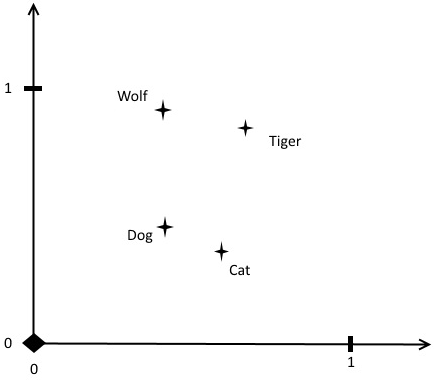
\includegraphics[scale=0.8]{msccls/explanatory_images/embedding_direction.png} 
\caption{Small example of a word embedding space. From \citet{franoischollet2017learning}.}
\label{fig:direction}
\end{figure}


In Figure \ref{fig:direction}, the four words \textit{cat}, \textit{dog}, \textit{wolf} and \textit{tiger} are represented on a geometric plane. We can clearly see some of the possible geometric transformations possible by using direction as a tool. For instance, the same vector that takes us from \textit{dog} to \textit{wolf} also takes us from \textit{cat} to \textit{tiger}. This could be interpreted this vector as ``converting a domesticated animal to its wildlife equivalent''. 

Another vector will take us both from \textit{cat} to \textit{dog} and from \textit{tiger} to \textit{wolf} which could be interpreted as ``converting a feline to a canine''. Two meaningful transformation vectors that are common in the real world are ``gender'' and ``plural'' vectors. By applying a ``female'' vector to \textit{king}, \textit{queen} is obtained and the same vector returns \textit{actress} if instead used on \textit{actor}. ``Plural'', as should seem obvious by now, if used on \textit{actor} will return \textit{actors}. 

Typically there are thousands of these types of interpretable direction vectors in a large word embedding.

\subsection{RoBERTa}








%Pytorch
%GRU
%Context-based 
%Commonsense Features
%Förklara bilden




%\section{Theory}
%NLP technique, categorization, ML, supervised/unsupervised,  
%Mechanical turks to 
%Finns både text och audio på MELD, \citep{zhang2019modeling} visar att text för sig är bättre än ljud men att text+ljud > text
%train, dev(validation), test, man testar på dev under development, först på test efter man är klar

\chapter{Implementation}
%Summary of what the chapter is about
This chapter is mainly focused on giving a clear description of what we have done for the duration of the project. Firstly we will describe the model that we used as a baseline, \textit{COSMIC}. Following, we will cover our model \textit{CASTLE}, how it has been implemented and what changes were made from COSMIC. Lastly, we will describe our setup and what corpora we used. 
%??In your text, you present COSMIC first. Change your intro so that it corresponds to your text??. 

We based our research strategy on the work by \citet{bouthillier:hal-02447823} that summarizes and reviews the experimental procedures that are most commonly used in the field of machine learning.

\section{Baseline -- COSMIC}
When trying to improve existing results in many machine learning fields, instead of starting from scratch, a baseline is used. A baseline is an already functioning model that provides basic results to the problem at hand. This provides the opportunity to allocate resources on improving the model instead of building it from the ground up and allows the machine learning community to expand on and draw benefits from each other's work. 

This project has been developed using the COSMIC model \citep{ghosal2020cosmic} as a baseline. COSMIC is a GRU-based model implemented with PyTorch that has achieved state-of-the-art results across four corpora commonly used in emotion recognition. The idea behind the model is when classifying an utterance, the emotions of the utterances both preceding and succeeding it are also taken into account. This way the context of the conversation can be used to more accurately predict the emotions of individual utterances. 


%COMSICs arkitektur bygger på att de skapar egna GRU-celler och GRU-lager som bygger på PyTorchs respektive. 
%Filip


Figure \ref{fig:COSMIC_arch} provides a simplified description of how COSMIC operates in a conversation between person A and person B. For each time step $t$ there is an utterance said by either A or B with the other person as a listener. At the next time step $t+1$ the roles are alternated. For each utterance, there exist multiple GRU-cells that predict both the intent of the speaker and the response of the listener at a certain time step. These cells are used not only to predict the emotion of the current utterance, but also used for the prediction of emotions in other utterances related to said utterance. 

COSMIC makes use of five different states to determine what emotion to predict. 
The four following states interact heavily with each other in a codependent manner. 

\begin{itemize}
    \item \textit{Context state} is a state shared between speaker and listener. It manages the current overall emotional state of the conversation. Affects both the Internal and External state.
    \item \textit{Internal state} tracks for each participant what emotions they are feeling but not necessarily showing. Affects the Intent state and the Context state.
    \item \textit{External state} portrays for each participant what emotions they are expressing to the other participants through both utterances and reactions. Affects the Context state.
    \item \textit{Intent state} is a state only present for the current speaker. As the name suggests, it represents the speaker's objective is for the current utterance. For example, if paying the listener a compliment, the intent could be to make the listener happier. This does not affect any other of the three states.
\end{itemize}
Internal state and External state are especially codependent as they combine into the sum of a participant's emotional state. 

The final state, Emotion state, takes into account the current utterance, the summed emotional state through the Internal and External state, as well as the Intent state to ultimately make a prediction for the current utterance. This process is repeated for every utterance in every conversation in the corpus.

%Softmax, relu mm


\begin{figure}[!ht]
    \centering
    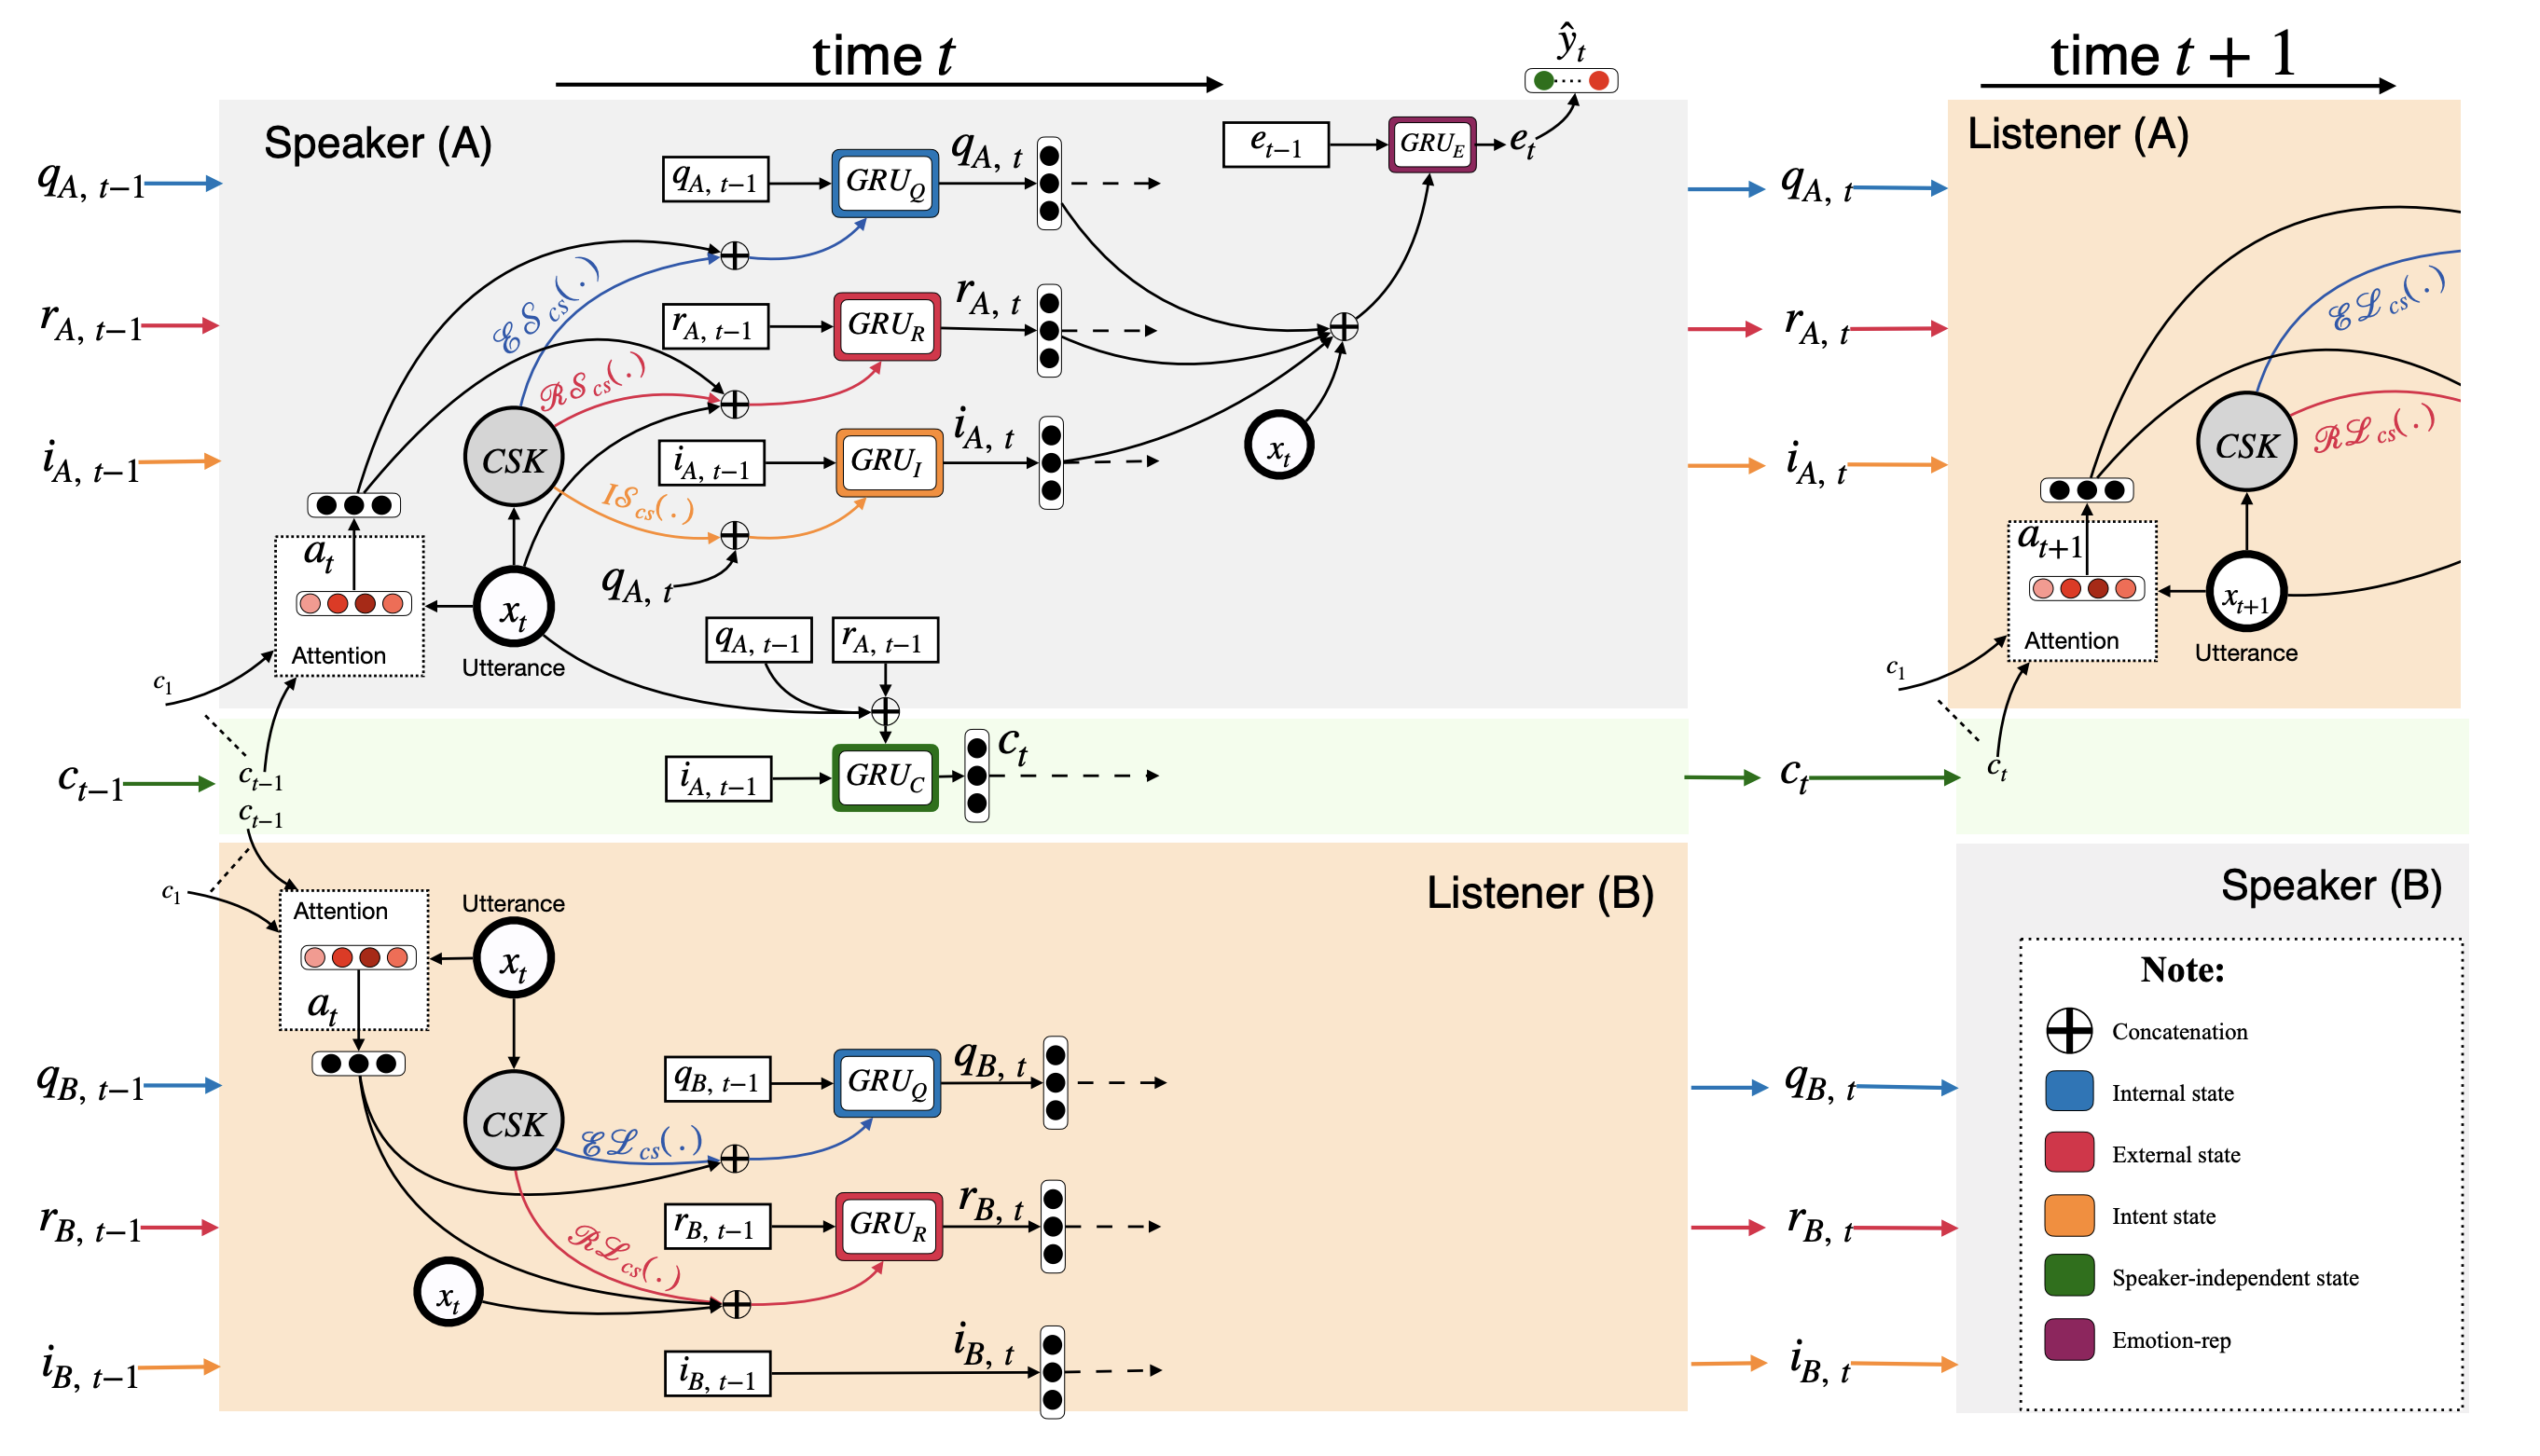
\includegraphics[scale=0.3]{msccls/explanatory_images/COSMIC_arch.png}
    \caption{COSMIC architecture. From \citet{ghosal2020cosmic}.}
    \label{fig:COSMIC_arch}
\end{figure}

%?? You could write a bit more on COSMIC ??

\section{CASTLE}
Building on COSMIC, we designed CASTLE, COSMIC-based AnalySer Taking advantage of LSTM for Emotion recognition, to answer our research questions. We have made several improvements on the COSMIC baseline, one of the fundamental being replacing the internal GRU architecture with an LSTM-based architecture as the name of the model indicates. 

At the start of the project, we read some recently published research in the field of deep learning, mainly the article by \citet{edseee.922172720200601} that states that GRU is not as suited for small pieces of text and large corpora as LSTM. This is where we got the inspiration to test whether or not the architectural change to LSTM could improve the results. 


COSMIC takes advantage of the \texttt{cudnn} framework in PyTorch to assist in multiple ways such as the \texttt{backends.cudnn.benchmark} which attempts to automatically optimize the algorithm during runtime. As we aimed to obtain as much control as possible over how the model behaved, we excluded this and other third party features that restricted our domain of control.  

COSMIC is also implemented with a \textit{residual} connection \citep{he2015deep} which allows the model to redefine the layers as learning residual functions referencing the layer inputs. This is supposed to facilitate the training of the model. While we originally wanted to implement this feature in CASTLE, there was simply not space to do it within the scope of the project. 


%Didnt implement residual for CASTLE tidsbrist

%Removed CUDA Backend since we wanted as little noise as possible interfering with our model We didnt want the reason for the results to be out of our reach. Third party. 


%COSMIC-based AnalySer Taking advantage of LSTM for Emotion recognition





\section{Experimental Setup}

%We chose COSMIC as our baseline because SOTA, more experienced in PyTorch
\subsection{Hyperparameters}
CASTLE's performance depends on three different hyperparameters. The ones we chose are \textit{dropout}, \textit{batch size}, and \textit{learning rate}. \citep{hyperparameters}:
\begin{enumerate}
    \item Dropout is a value between 0 and 1 that regulates what percentage of learned data that the model randomly chooses to forget. This is used in order to combat overfitting and make sure the model is actually predicting instead of just learning the structure of the corpus.
    \item  Batch size governs how many training examples will be utilized in each iteration. A larger value increases the accuracy of the gradient in trade off for a higher memory cost.
    \item  Learning rate defines the speed of which the model updates its parameters. A high learning rate speeds up the learning at the risk of not converging while a low value will more likely converge, sacrificing speed in the process.
\end{enumerate}

To optimize our hyperparameters, we implemented the \texttt{Tune} framework offered by \texttt{Ray}. This framework allowed us to efficiently experiment with many different configurations and provided a simple way to run trials concurrently. Most of our optimization were done with a combination of grid search and random search. Random search is a function with two parameters \textit{start} and \textit{end}, and for each trial it randomly selects a float from in between the two values to use for the given hyperparameter. Grid search instead takes in a list of floats as a parameter and runs a trial for each value in the list. Multiple grid searches can very easily take a large amount of time to run as all possible combination of values across all grid searches will be tested in separate trials. 

Our approach was to start out with random search on parameters to get a sense on what range of values produced optimal results. Once we had established the magnitude of which we wanted our parameters to be, we tested out various combinations with grid search, keeping the ones that produced promising results and replacing the others with new trials.


\subsection{Comparison with Current Practices}
When deciding what configuration to use for our experiments, we based our decisions on the empirical studies made by  \citet{bouthillier:hal-02447823}. In their report, they surveyed authors whose papers were presented at the peer-reviewed conferences NeurIPS 2019 and ICLR 2020. As the work is based on answers from relevant authors in the machine learning community, we found it appropriate to use the answers as guidelines for our setup. Instead of relying on our own intuition, basing it on the broad consensus grants the experiment a certain sense of validity. In Figure \ref{fig:HAL}, we have presented the questions and responses we took into consideration.

CASTLE is fine-tuned on three hyperparameters where a combination of \textit{grid search} and \textit{random search} was used. On average, we performed 20 sets of different values for the three hyperparameters across all corpora. CASTLE was intended to be evaluated on four different corpora but ultimately only provided results for three of them. Our results are based upon 10 consecutive runs with the same setup. 

Comparing this to the responses observed in \ref{fig:HAL}, we are in line with the majority in all but one instance, (f), where the majority base their results on 5 or less samples and we instead chose to base it on 10 samples as a higher sample size tends to become a more reliable result.

\subsection{Equipment}
As for our hardware setup, we were not able to run and train the model on our laptops as they lack a GPU. To execute our code, we instead utilized Google Colab, a cloud based service where users can remotely run their code on Google servers that are built with more powerful hardware and can handle high demand programs such as machine learning model. Using a remote service proved to be perfectly fine for three of the four corpora we aimed to run our model on. The fourth one, \textit{DailyDialog}, unfortunately required more memory than we were allocated and could not complete run.


%Hur vi "räknade ut" våra resultat, 10 avg på best valid ->( test)
%Epochs
%Google Colab
%Ray Tune för att studera hyperparametrar och automatisera
%HAL - diskussion


%How many sets of hyperparameters we evaluated? Vi hade i snitt 20:ish per dataset
%4 dataset for the experiment
%Reported 10 samples as one averge. 

%Stycke där vi jömför med HAL

\begin{figure}[!ht]

\centering
\subfloat[Did you optimize your hyperparameters?] {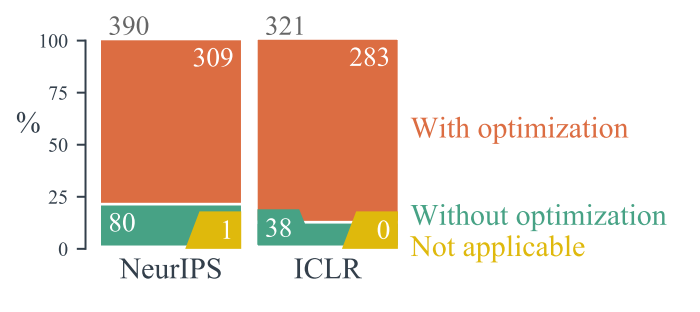
\includegraphics[width=\linewidth/2]{msccls/Questionnaire/Q2.png}}\hfil
\subfloat[If yes to (A), how did you tune them?] {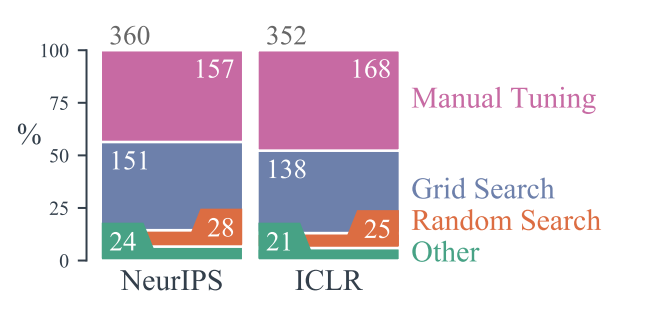
\includegraphics[width=\linewidth/2]{msccls/Questionnaire/Q3.png}}

\subfloat[How many hyperparameters did you optimize?] {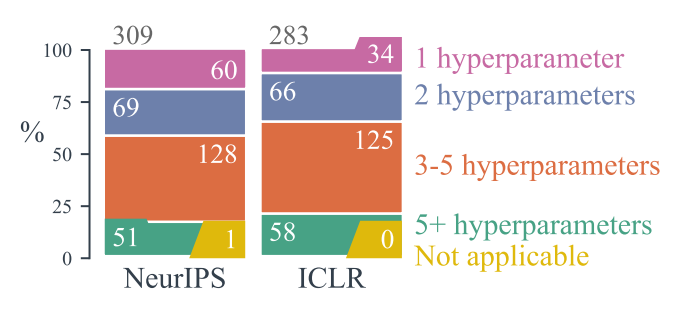
\includegraphics[width=\linewidth/2]{msccls/Questionnaire/Q4.png}}\hfil  
\subfloat[How many trials/experiments in total during the optimization?] {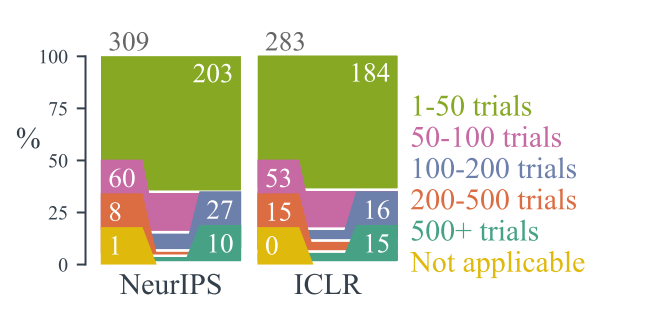
\includegraphics[width=\linewidth/2]{msccls/Questionnaire/Q5.png}}  

\subfloat[How many datasets or tasks did you compare on?] {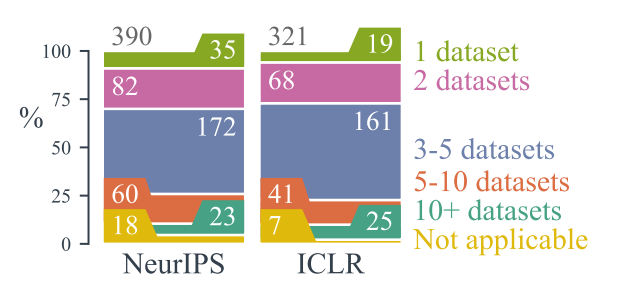
\includegraphics[width=\linewidth/2]{msccls/Questionnaire/Q8.png}}\hfil
\subfloat[How many results did you report for each model?] {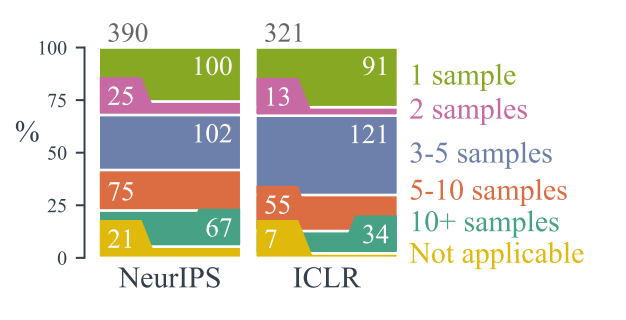
\includegraphics[width=\linewidth/2]{msccls/Questionnaire/Q9.png}}
\caption{Collection of questionnaire answers regarding machine learning experiments. From \citet{bouthillier:hal-02447823}.}
\label{fig:HAL}
\end{figure}








%Lack of resources


%Hyperparametrization with Tune
%Learning rate
%Dropout
%Batch_size [RAM limitations]
%Definitioner finns redan i terminologi
\section{Corpora}

To evaluate our model, we used four popular corpora that are frequently used in emotion recognition research work. We chose these corpora as we wanted our results to be comparable with the current state-of-the-art, namely COSMIC as well as the common practice observed in Figure \ref{fig:HAL}(e). As COSMIC compared its results to several other models using these corpora, the results of CASTLE will be directly comparable with COSMIC and the other models. 

All the following corpora include a \textit{neutral} emotion that is not very descriptive. An emotion is classified as neutral when it can not be classified as any of the other emotions. Each corpus uses its own set of emotions and method of classification to label said emotions. 
%mention mechanical turks as example? [MELD?]

%Ranges in size
%These datasets are recurring in many of the papers on this subject. -> our results comparable
%All these data sets include a "neutral" emotion. This is when an emotion couldn't fit into any of the other categories within the data set using their corresponding methods for classifying the emotions. 
%Fyra populära dataset inom NLP

%train-valid-test i vårt fall

\begin{description}
    \item[MELD] \citep{poria2019meld} is based on about 13,000 utterances and 1,400 dialogues from the TV series \textit{Friends} and is an extension to the EmotionLines dataset \citep{chen2018emotionlines}. MELD is multimodal and  frequently has more than two speakers per dialogue. The utterances are labeled with the following emotions: \textit{anger}, \textit{disgust}, \textit{sadness}, \textit{joy}, \textit{surprise}, \textit{fear}, and \textit{neutral}.

    \item[IEMOCAP] \citep{busso2008iemocap} is a multimodal, multispeaker corpus with utterances from acting and improvisation scenarios emphasizing on emotional expressions. The utterances are labeled with the following emotions: \textit{anger}, \textit{happiness}, \textit{excitement}, \textit{sadness}, \textit{frustration}, \textit{fear}, \textit{surprise}, \textit{other}, and \textit{neutral state}.
    
    \item[EmoryNLP] \citep{zahiri2017emoryNLP} is also a corpus with transcripts from the TV series \textit{Friends}. In comparison to MELD, EmoryNLP has over 60,000 utterances. The utterances are labeled with the following emotions: \textit{neutral}, \textit{joyful}, \textit{peaceful}, \textit{powerful}, \textit{scared}, \textit{mad} and \textit{sad}.
    
    \item[DailyDialog] \citep{lietal2017dailydialog} encompasses numerous daily life topics with human-written dialogues to reflect usual day-to-day conversations. The corpus has an average of circa 8 speakers per dialogue and has a total of over 13.000 dialogues with their emotions manually labeled. The utterances are labeled with the following emotions: anger, disgust, fear, joy, neutral, sadness, and surprise.
\end{description}


Following are sample dialogues from two of the corpora to showcase how the speakers, dialogues and their respective emotions are structured. Additionally, we want to demonstrate the difference in topics of the dialogues that might be important to notice when selecting a corpus for a problem. 

\subsection{Corpus Structure}
Each of our corpora are structured similarly. They contain a training set, a test set, and development set, usually shortened to dev or val (for validation). These sets are all structured identically and containing utterances randomly selected from the full corpus, with the bulk of the utterances in train, and test and val of approximately the same size. As the name implies, the training set contains the data that the models sets out to train on. The other two are used together to produce our results. While the test set is where we get our results from, we do not want to directly access our results from it as there is a risk that we accidentally manually overfit our model when tuning it based on our intermediate results. Instead, the result that gets reported is the F1 score in the test set for the epoch where the dev set produced the best F1 score. 


\subsection{Corpus Excerpts}
\label{corpus_excerpts}
\paragraph{MELD.} The annotated emotions in MELD are chosen by the majority verdict of five independent \textit{Amazon mechanical turks}. Each one of these are tasked to manually examine utterances one by one and then select what emotion out of the options is most suited for that utterance.
%?? Here have afew intro words as for IEMOCAP ??
\newenvironment{pag}{\fontfamily{pag}\selectfont}{\par}


\begin{table}[H]
    \begin{pag}

    \centering
    \begin{tabular}{lll}
Rachel: & Thank you. Oh Joey and look at this crib! It's so cute! & \textit{Joy} \\
Joey: & I know! I found it on the street. & \textit{Joy} \\
Rachel: & Are you serious, Really?! It's in such good condition. & \textit{Surprise} \\
Joey: & Yeah. & \textit{Neutral} \\
Rachel: & Wow! Whoa-whoa what's under the covers? & \textit{Surprise} \\
Joey: & I don't know. & \textit{Neutral} \\
Rachel: & It's moving. & \textit{Fear} \\
Joey: & Ew. & \textit{Disgust} \\
Rachel: & It's still. It's got a tail! Get it out of here! Get it out of here!! & \textit{Fear} \\
Joey: & Ooh! Ah! Okay! & \textit{Fear} \\
    \end{tabular}
    \label{tab:dialogue_meld}
\end{pag}
\end{table}

\paragraph{IEMOCAP.}
IEMOCAP determines the emotion of an utterance through the response of four independent observers. If the observers can reach a clear consensus, that consensus is chosen as the motion, otherwise, it is put as undecided.  

\begin{table}[H]
    \begin{pag}

    \centering
    \begin{tabular}{lll}
Female: & Uh-, So I got some good news. & \textit{Happiness} \\
Male: & You're not pregnant or anything. & \textit{Neutral} \\
Female: & Pregnant? What are you talking about? No. & \textit{Surprise} \\
Male: & I know you've been trying to have a baby, right? & \textit{Neutral} \\
Female: & I have some better news than that. & \textit{Happiness} \\
Male: & Oh, really? & \textit{Undecided} \\
    \end{tabular}
    \label{tab:dialogue_iemocap}
\end{pag}
\end{table}

%female 2ggr för olika känslor mitt i dialog








\ifx false
Subject to removal
Filip
\subsection{Approach} 
\section{Method}
Google Colab
Word level one hot encoding, kanske relevant, avgör beroende på hur mycket mer vi behöver skriva.
\section{Implementation}
Overfitting \\
Data Augmentation \\
importance of finding the correct data-sets \\
\section{Bibtesting, will be removed}
\citep{emotionlinesdataset} \\
\citep{franoischollet2017learning}\\
\citep{beaver2020towards}

\fi

\chapter{Results}
\label{result_chapter}

% Please add the following required packages to your document preamble:
% \usepackage{multirow}
\begin{table}[!ht]
\begin{center}
\begin{tabular}{lcccc}
\hline
\textbf{W-avg F1 score} & \textbf{MELD}           & \textbf{IEMOCAP}        & \textbf{EmoryNLP}  \\ \hline
KET                     & 53.37           & 59.56          & 34.39 \\
CNN                     & 55.02           & 52.04          & 32.59 \\
DialougeRNN             & 57.03           & 62.57          & 31.70 \\
DialogXL                & 62.41           & 65.94          & 34.73 \\
COSMIC                  & 65.21           & 65.28          & \textbf{38.11} \\ \hline
CASTLE                  & \textbf{65.27} & \textbf{66.13} & 37.86\\ \hline
\end{tabular}
\end{center}
\caption{Comparison of the weighted average F1-score between CASTLE and other models taken from \citet{ghosal2020cosmic} and \citet{Shen2020DialogXLAX}. State-of-the-art results in bold. }
\label{results_table}
\end{table}

As Table \ref{results_table} shows, CASTLE achieves state-of-the-art results for both the MELD and IEMOCAP corpora. While not producing state-of-the-art results for EmoryNLP, CASTLE manages to produce a score within 99$\%$ of the current state-of-the-art.


%Ha samma storlek på tabellerna



\ifx false
\begin{table}[h!]
\begin{tabular}{|c|c|c|c|c|}
\hline
Time per epoch & MELD             & IEMOCAP          & EmoryNLP          \\ \hline
COSMIC         & XXX s            & XXX s          & XXX s                  \\ \hline
CASTLE         & \textbf{46.16 s} & \textbf{27.10 s} & \textbf{43.02 s}       \\ \hline
\end{tabular}
\end{table}
\fi

%As we can see CASTLE obtains sota
%Prata om att dessa resultaten är state-of-the-art och vad det innebär


%These are our results


\chapter{Discussion}
In this chapter we start by analyzing the results that CASTLE achieved. Consequently, the limitations that impeded the project will be mentioned and discussed. Finally we will mention in what ways the project can further be explored. 



%We compare our results to the other baselines results that COMSIC presents in their report.
%When we started working with the project our main goal was in creating that produced state-of-the-art results 


%\section{Discoveries}

\section{Performance}

As stated in the \nameref{result_chapter} Chapter, CASTLE accomplishes state-of-the-art results in multiple corpora annotated for emotion recognition. This makes the case for CASTLE being an improvement over current state-of-the-art models, namely COSMIC for MELD and DialogXL for IEMOCAP. EmoryNLP was the only corpus that we managed to run CASTLE on without achieving state-of-the-art results. 

There might be several reasons for this but we believe that one of them is more likely than the others. As EmoryNLP was the last corpus that we optimized CASTLE for, there was not enough time to thoroughly tune the hyperparameters. The method we used for optimizing hyperparameters was to initially use random search to find relevant sets of parameters, where the leading values were then iterated through with the help of grid search. 

Working in this way is somewhat of a scattershot approach where we depend unpleasantly much on the results of random searches. While the random searches clearly produced competitive results, there is nothing to indicate that whether or not an optimal set of values was overlooked. Since CASTLE produces results within 99$\%$ of current state-of-the-art, it is our belief that with additional time and resources CASTLE could produce state-of-the-art results for EmoryNLP as well. 

The evidence demonstrates that CASTLE outperforms its competitors on the MELD and IEMOCAP corpora while remaining competitive on EmoryNLP and with inconclusive results for DailyDialog. This fulfills the primary aim of our thesis that we defined in section \ref{research_questions} and makes CASTLE one of, if not, the most viable systems to adapt for practical emotion recognition applications.

The primary improvement we implemented was replacing an existing GRU layer with a more complex LSTM one. As mentioned earlier, the theory states that LSTM layers is likely to outperform GRU layers, when there is enough data, at the expense of computation power. Since LSTM is a more complex structure with an additional gate as well as having the concept of utilizing memory in a cell state, it is no surprise that it has the potential to outperform GRU layers. When debating if to use CASTLE or some other model, it would boil down to whether or not increase in certainty is worth the cost in computational power. 




%adding feautrés costs resources and time

%Vårt main mål var att förbättra performance med LSTM.
%Kan inte skriva förrän state-of-the-art på Emory
%Our results are the average of  10 samples since we wanted them to be comparable to COSMICs. 
%Avvägning mellan performance och tid


%Changed architecture for increased performance, then focused primarily on reducing runtime
%LSTM är enligt teorin vi har läst bättre men tar längre tid
%LSTM är en mer avancerad design. Leder ofta till bättre men tar längre tid. Tar upp mer resurser


\section{Limitations}
\label{limitations}

At the start of this project, the scope was a lot larger than the one explored during this thesis. Originally the model was intended to also perform keyword extraction in addition to emotion recognition. This was based on discussions with Telavox, where the idea was a model that could identify the topic of the conversation and the emotions of the parties involved. Unfortunately, a corpus fitting for this task does not exist at this time. This meant that in order to fulfill the original scope, we would have to both create and annotate such a corpus. Such a task could be considered a master's thesis by itself and certainly was not possible to complete in tandem with creating a model, at least not in the given time frame. As the project is only intended to run for 20 weeks, we had to make a decision about how to proceed and we decided that a model producing state-of-the-art results but not in customer service would be more rewarding, for both us and Telavox, than a specialized customer service model providing average results. 

When deciding the scope, we also underestimated just how time consuming this project was going to be. The initial thought of both emotion recognition and keyword extraction, even with a specialized corpus available from the start, would be a difficult challenge to complete in the time frame. As we feel that more time could have been spent on optimization with potential better results for EmoryNLP, adding a wholly new task in the form of keyword extraction would most likely have produced lacking results for both tasks.

As the laptops we were using did not contain a GPU, running our code locally was not possible and we were instead bound by the rules of Google Colab. One of these rules is that no notebook can run for more than 24 hours straight. Hyperparameter optimization is a time consuming task that is solved by trial and error, and this restriction meant that we could not run as many trials at a time as we wanted which in turn led to less optimization as there simply was not enough time.


%Tid på Colab max 24h
%Tid på exjobb max 20 veckor
%Tid för hyperparametrization
%Reducerat scope. Ju mer överdrivet desto bättre. Vi tänkte från början ha recognition OCH keyword extraction. Speech-to-text. Vårt originalscope baserades på att vi hade ett privat dataset att jobba på t.ex. telekom. 
%Kan inte köra ML på våra datorer pga ingen GPU -> kör på cloud
%real time translation
\subsection*{DailyDialog}
%No resources available to run this with LSTM 
Originally we intended to have CASTLE run on the same corpora that COSMIC produced results for. However, due to the previously discussed hardware limitations, we did not have enough memory to run CASTLE on DailyDialog. Despite continuous attempts at optimization, we were unable to complete a finished run with the corpus and instead repeatedly ran out of memory. 

The reason for this is twofold. Firstly, DailyDialog is close to a magnitude larger than the other corpora used in this experiment. Secondly, LSTM is a complex architecture with more gates and calculations which leads to higher demand in hardware. As Google Colab has a limited amount of memory for us to utilize, we did not have to option to run the corpus on the service. On the other hand, with access to more memory, there is a great possibility that we would produce close to, if not, state-of-the-art results for DailyDialog as well. 

\section{Future Work}


Considering the fact that CASTLE did not produce state-of-the-art results for the EmoryNLP corpus, the most natural continuation for the project is to have CASTLE achieve this goal. Our proposal is to simply spend more time with hyperparameter optimization and explore what results that might provide. Even though CASTLE managed to achieve state-of-the-results for MELD and IEMOCAP, an extensive hyperparameter optimization could possibly improve the results further.  

%DailyDialog? 

Another natural continuation for the project is to expand the scope to what it initially was defined as. As stated in \nameref{limitations}, the initial goal of the project was to create a model for analyzing written customer service conversations and using keyword extraction as a complement to said analysis. CASTLE could very well be used as a framework for completing this type of task.


CASTLE is undoubtedly able to analyze written conversations with great success. However, the corpora used for training CASTLE are not completely suited for customer service specific dialogues. When searching for appropriate corpora, there was no customer-service themed corpus annotated with emotions available. One possibility is to create such a corpus using an already existing unannotated customer service related corpus and labelling it with emotions. A couple of methods has previously been mentioned in section \nameref{corpus_excerpts} for how a corpus can be annotated with emotions. 


In the same manner that CASTLE built upon the work of COSMIC, other projects can achieve even better results by building upon CASTLE. 



%som vi nämner i limitations 


%Utöka scope till vad det var från början vilket var, emotion recognition i samtal. Både i realtid och transcribed calls. Keyword extraction kan användas som ett supplement. 
%Skapa ett dataset specifikt för customer service
%Ytterligare ändringar som kan ge state-of-the-art
%Mer utförliga hyperparameter optimization. 




\chapter{Conclusions}
When we started this project, our goal was to find answers to the research questions mentioned in section \ref{research_questions}. After completing this project, it is safe to say that creating a model capable of fulfilling our primary aim was possible, as CASTLE is just that. CASTLE also proves that an LSTM architecture can in fact outperform a GRU one. When comparing CASTLE to the previous state-of-the-art models we show, as presented earlier, that CASTLE surpasses those models. Our secondary aim and last research question unfortunately has to remain unanswered due to time limitations. All in all, we consider CASTLE a success as it produces state-of-the-art results for two corpora and has the potential of achieving it for the remaining two as well, thus fulfilling our primary aim.  

%Able to produce 


% Should use consistent formatting when it comes to Names ("FirstName LastName", or "F. LastName")
%\printbibliography
\makebibliography{MyMSc}

\begin{appendices}
\chapter{Dummy Appendix}






% display used packages information unless nofilelist is used in the cslthse-msc package option
\printfilelist

%make sure we're on even page with the pop-sci
\checkoddpage
\ifoddpage
\else
   \newpage
   \thispagestyle{empty}
   \mbox{ }
\fi
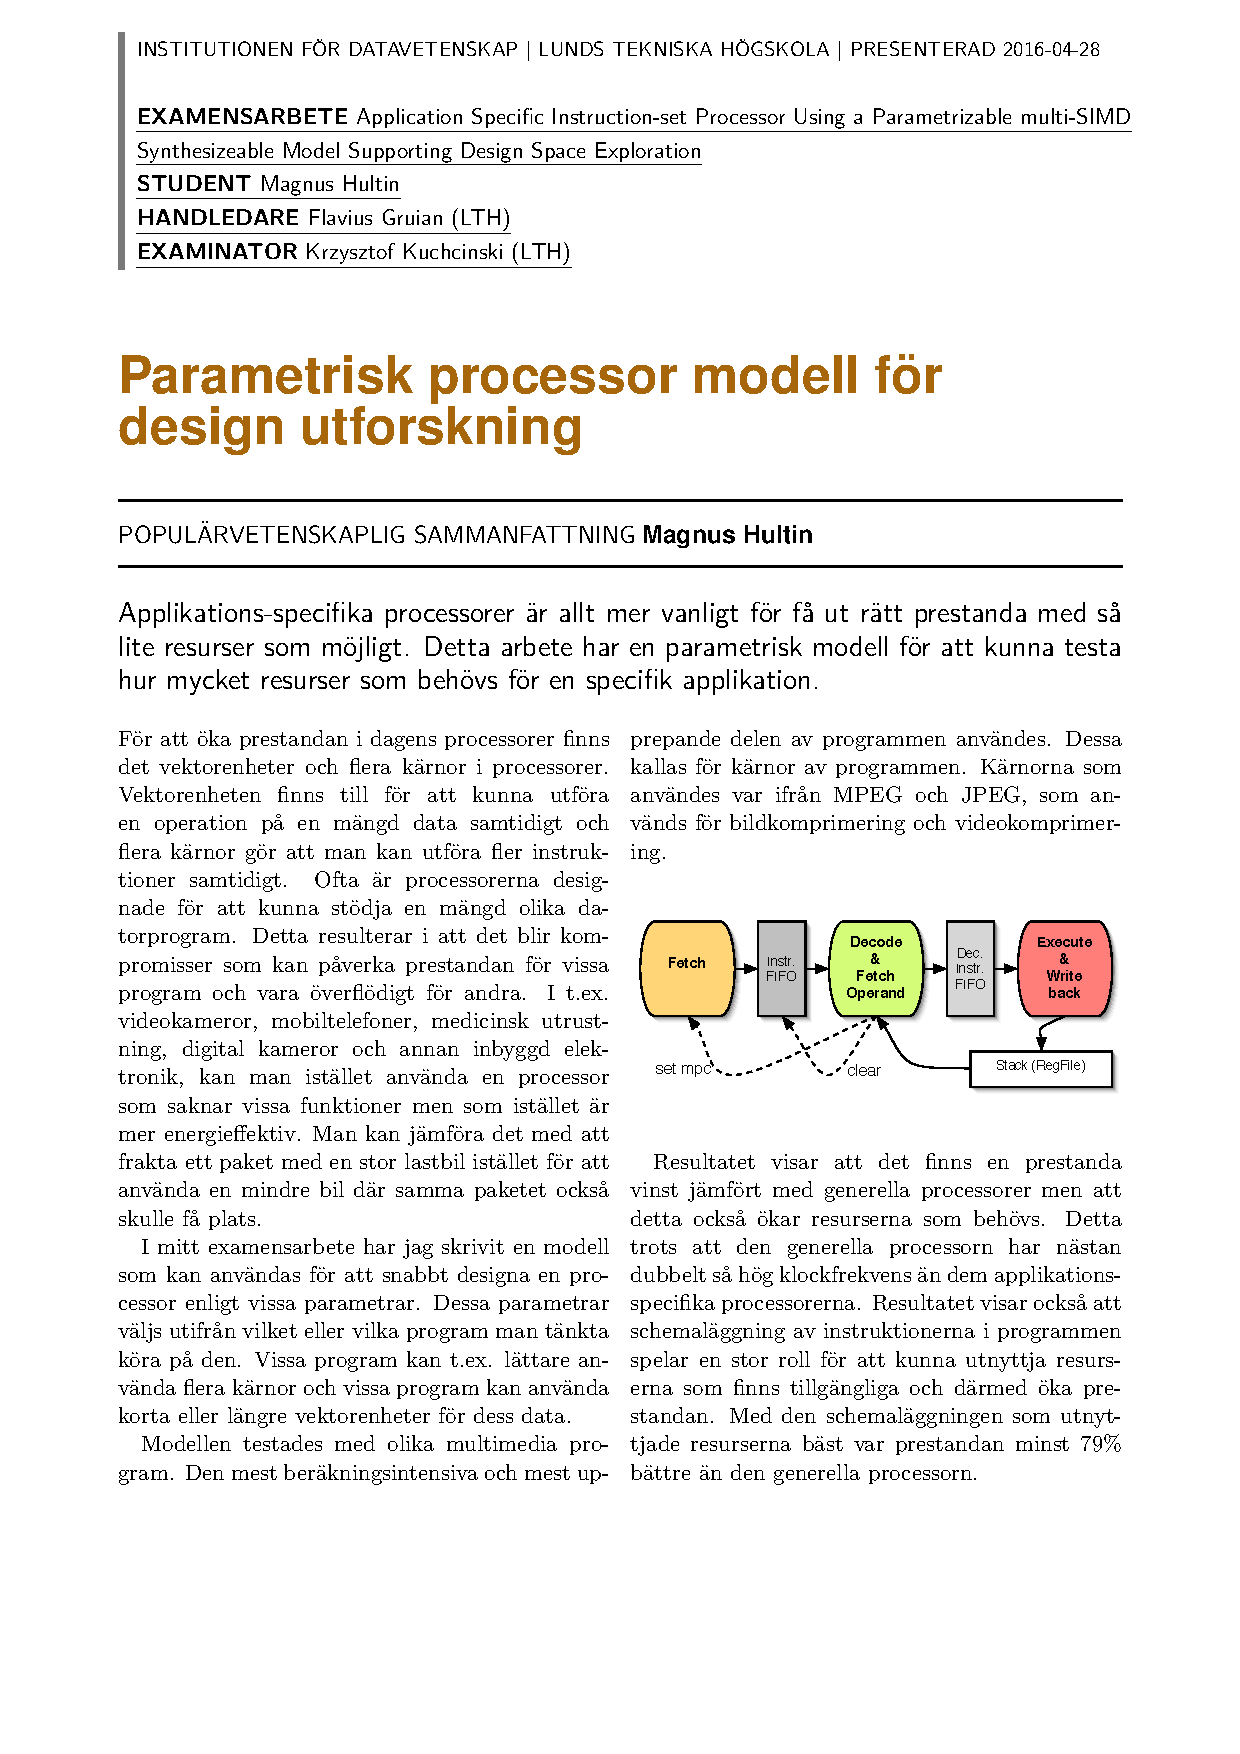
\includepdf[pages={1}]{popsci/popsci.pdf}
\end{appendices}

\end{document}